\documentclass[a4paper,12pt]{article}
\usepackage[T1]{fontenc}
%	Choose font encoding with support for extended characters.	
\usepackage[utf8]{inputenc}
%	Allow utf8 input. Has to match encoding of the file.

% ======
% Layout
% ======

\usepackage[left=3cm, right=3cm, top=2.5cm, bottom=2.5cm]{geometry}
\setlength{\headheight}{14.5pt}
%	Enlarged headheight because of a fancyhdr warning


% ======
% Tables
% ======

\usepackage{ltablex}
%	Modifies the tabularx environment to allow for display breaks. 

\keepXColumns
%	Necessary to keep the tables aligned to the left.

\setlength\LTpre{0pt}
%\setlength\LTpost{0pt}
%	Vertical space before and after tabularx

% ============
% Bibliography 
% ============

\usepackage{biblatex}[bibstyle=authortitle]
\addbibresource{./bibliography/bibliography.bib}
%\defbibenvironment{midbib} 
%  {\list
%     {}
%     {\setlength{\leftmargin}{\bibhang}%
%      \setlength{\itemindent}{-\leftmargin}%
%      \setlength{\itemsep}{\bibitemsep}%
%      \setlength{\parsep}{\bibparsep}}}
%  {\endlist}
%  {\item}
% Suppress the numbering in bibliography

% ===================
% Headers and footers
% ===================

\usepackage{fancyhdr}
\pagestyle{fancy}
\lhead{P. H\'ajek, Academic CV}
\rhead{\today}
\cfoot{\thepage}

% =========
% Formating
% =========

\usepackage{libertine}
%	Font
\usepackage{titlesec,xcolor}
\titleformat{\section}{\color{olive}\normalfont\scshape}{}{}{} 
%	Customization of sections headings.
\def\arraystretch{1}
%	Vertical stretch of tables.
\setlength\parindent{0pt}
%\setlength\parskip{0pt}

% ===================
% Additional packages
% ===================

\usepackage{hyperref} 
%	href,...
\usepackage{graphicx}
%	includegraphics,...
\usepackage[export]{adjustbox}
%	valign in includegraphics
\usepackage[inline]{enumitem}
% 	better control of enumerate,...
\usepackage{amssymb}
%	\mathbb, \mathbf,...
%\usepackage{filecontents}
%	For writing bibliography directly in the file.
\usepackage[final]{microtype}
%	For better typeseting, solves some overflows in the bibliography, etc...

% ===============
% Custom commands
% ===============

\begin{document}
%
% ============
% Contact data
% ============
%
\begin{minipage}[t]{.7\textwidth}
	{\Large Pavel H\'ajek}\\[.2cm]
	Hackerova 791/1\\
	181\,00, Prague 8, Czech Republic \\[.2cm]
	%University of Hamburg\\
	%Bundesstra\ss e 55 --- Geomatikum\\
	%20\,146 Hamburg, Germany \\[.2cm]
	Phone: +49 176\,995\,71920\\
	Email: \href{mailto:hajek_pavel@yahoo.de}{hajek\_pavel@yahoo.de}\\[.2cm]	
	Born on September 29, 1987 in Prague\\
	Nationality:  Czech\\[.2cm]
	Personal website: \href{https://p135246.github.io}{https://p135246.github.io}
\end{minipage}
\hfill
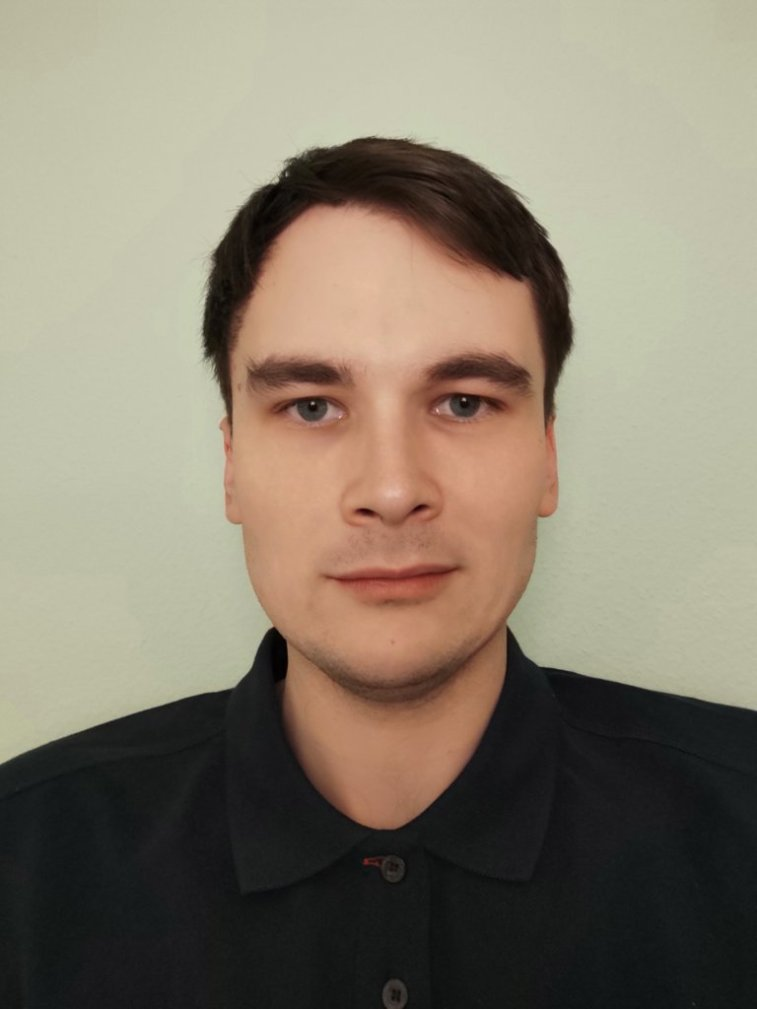
\includegraphics[scale=0.13,valign=t]{./graphics/me-120121.jpeg}
%
%=============================
\section*{Academic positions}
%=============================
%
\begin{tabularx}{\textwidth}{@{}lX@{}}
	Jan--Feb 2021 	&\emph{Guest researcher} in the symplectic geometry group of Prof.~Dr.~Chris Wendl at the Humboldt University of Berlin.\\
	Sep--Dec 2020 	&\emph{Mittag-Leffler scholar} in the program "Knots, strings, symplectic geometry and dualities". \\
	Oct 2019--2021 &\emph{Postdoc} with specialization in string topology and symplectic geometry with Prof.~Dr.~Janko Latschev at the University of Hamburg.

			(position interrupted until March 2021)
\end{tabularx}
%	The @{} are added so that no additional space is added before the first and after the last column.
%
%=============================
\section*{Research interests}
%=============================
%
\begin{description}[font=\normalfont\itshape,itemsep=0pt,parsep=0pt]
	\item[Actively:] Chain models of string topology coming from symplectic geometry (moduli spaces of holomorphic curves), understanding relations to Chern-Simons theory, TCFT's and string field theory, applications of the language of operads, applications of the BV-formalism.
	\item[Generally:] Symplectic geometry, string topology, dynamical systems---spinning tops and celestial mechanics, symmetries, integrability and semi-classical physics, mathematics of QFT and string theory.
	%(e.g., work of E. Witten and P. Nev). 
\end{description}
%	Setting normal font is needed to have the item caption in normal font. 
%
%====================
\section*{Education}
%====================
%
\begin{tabularx}{\textwidth}{@{}lX@{}}
	2015--2019 & \emph{PhD in Mathematics supervised by Prof.~Dr.~Kai~Cieliebak at the University of Augburg.}
	
			\href{https://opus.bibliothek.uni-augsburg.de/opus4/72493}{Thesis} on IBL-infinity algebras, string topology and perturbative Chern-Simons theory.
			Training in symplectic topology and dynamical systems.
			Final grade Magna cum laude.\\
	2011--2014 & \emph{MSc in Theoretical and Mathematical Physics, LMU Munich.}
		
			Thesis on Eilenberg-Steenrod axioms for a homology theory based on manifolds with corners supervised by Prof.~Dr.~Kai~Cieliebak.
			Graduated with high distinctions.\\
	2007--2011 & \emph{BSc in Physics, Charles University in Prag.}

			Thesis on dynamical symmetries in classical and quantum mechanics supervised by prof.~RNDr.~Pavel Cejnar, Dr., DSc.
			Graduated with distinctions.\\
	2007--2010 &  \emph{BSc in Mathematics, Charles University in Prag.}

			Thesis on Liouville integrability of a generalization of the Lagrange top to higher dimensions supervised by doc.~RNDr.~Svatopluk~Kr\'ysl, Ph.D.
			Graduated with high distinction. 
\end{tabularx}
%
%=======================
\section*{Scholarships}
%=======================
%
\begin{tabularx}{\textwidth}{@{}lX@{}}
	Sep--Dec 2020	& 	Junior Fellowship from the Mittag-Leffler institute.\\
	2012--2013 	& 	Scholarship for master studies by the DAAD (full coverage). \\
	2007--2011 	& 	Merit based scholarship from the Charles University.
\end{tabularx}
%
%======================
%\section*{Publications}
%======================
%
%\begin{refsection}
%	\printbibliography[heading=none]
%\end{refsection}
%
%====================
\section*{Preprints}
%====================
%
\begin{refsection}
	\nocite{20PhD}
	\nocite{20Hodge}
	\nocite{19FirstLook}
	\printbibliography[heading=none]
\end{refsection}
%
%====================
\section*{Papers in preparation}
%====================
%
\begin{tabularx}{\textwidth}{@{}lX@{}}
	\textbullet	&	Chain-level equivariant string topology for simply connected manifolds (with K.~Cieliebak and E.~Volkov).\\
	\textbullet	&	Chain-level string topology for $\mathbb{S}^1$ (with K.~Cieliebak).\\
	\textbullet	&	Chern-Simons Maurer-Cartan element in various contexts (with L.~Peksov\'a).\\
	\textbullet	&	Vanishing results for Hodge propagators.
\end{tabularx}
%
%===================
\section*{Teaching}
%===================
%
\begin{tabularx}{\textwidth}{@{}lX@{}}
SS20 		& 	Exercise class in Floer Theory.\\
WS19 		& 	\textbullet~Four exercise classes in Mathematics for physicists I (German).\\
		&	\textbullet~Exercise class in Symplectic Geometry.\\
WS16--SS17 	& 	Teaching assistant in  Analysis I \& II (German).\\
SS16 		& 	Coorganizer of a seminar on Floer homology.\\
WS14--SS15 	&  	\textbullet~Teaching assistant in Linear Algebra~I \& II (German).\\
		&	\textbullet~Homework corrector in courses for math teachers (German).\\
SS12--WS13 	& 	Homework corrector for Algebraic Topology~I~\&~II. 		   
\end{tabularx}
%
%====================================
\section*{Other academic experience}
%====================================
%
\begin{tabularx}{\textwidth}{@{}lX@{}}
	2018 	& 	Help with organization of the \href{https://www.math.uni-augsburg.de/prof/geo/SFTIX/}{Workshop on Symplectic Field Theory IX,} University of Augsburg, August 25--31 (responsible for the webpage and videos).\\
\end{tabularx}
%
%======================
\section*{Talks given}
%======================
%
\begin{tabularx}{\textwidth}{@{}lX@{}}
2021		&	Chain models of string topology coming from symplectic geometry I~\&~II, Symplectic seminar of the Humboldt University of Berlin, January 11 and 25.\\
2020 		&	\textbullet~Symplectic chain models of string topology, Mathematical Institute of Charles University in Prague, December 17.\\
		&	\textbullet~Chern-Simons theory on $\mathbb{S}^1$ I~\&~II, Informal seminar at the Mittag-Leffler institute, Stockholm, September 16 and 21.\\
		&	\textbullet~$\mathrm{IBL}_\infty$ chain model of equivariant string topology from perturbative Chern-Simons theory, Seminar on Lie groups and moduli spaces, University of Geneva, June 16.\\
2019 		&  	\textbullet~Computations of the $\mathrm{IBL}_\infty$ structure, Workshop on String field theory, BV quantization, and moduli spaces, Simons Center for Geometry and Physics, Stony Brook, May 20--24.\\
		& 	\textbullet~Explicit computation of Feynman integrals, Seminar for symplectic geometry, University of Augsburg, May 13, 2019.\\
		& 	\textbullet~$\mathrm{IBL}_\infty$ formality and Poincar\'e duality models, Seminar for symplectic and contact geometry at the University of Hamburg, April 25.\\
		& 	\textbullet~Chern-Simons theory and string topology, Seminar of the Research Institute for Mathematical Science, Kyoto, March 14.\\
		& 	\textbullet~Feynman integrals with the Green kernel, Seminar of the Mathematical Institute at the University of Potsdam, February 28.\\
		& 	\textbullet~$\mathrm{IBL}_\infty$ structure and string topology conjecture, 39th Winter School Geometry and Physics, Srn\'i, January 12--19.\\
2016 		& 	Presentation of a part of the proof of the Cheeger-M\"uller theorem, Block seminar on Torsion in Geometry and Topology, Schloss Gollwitz, Brandenburg, July 3--8.\\
2015 		& 	Homology theory based on manifolds with corners,  Meeting of symplectic geometers, Weimar, Germany, 16--18 January.
\end{tabularx}
%
\emph{Some other talks in local seminars:}
\medskip
\begin{tabularx}{\textwidth}{@{}X@{}}
Costello's work on TCFT's, Chas-Sullivan string topology, Cyclic homology, Seiberg-Witten theory, Symplectic capacities and the ball packing problem, E.~Witten's non-perturbative treatment of Chern-Simons theory, Linking numbers and Green kernels, Dynamics near the Lagrange points in the restricted three body problem, Molecules of the Euler top.
\end{tabularx}
%
%==============================
\section*{Conferences attended}
%==============================
%
\begin{tabularx}{\textwidth}{@{}lX@{}}
2020 	& \href{http://conference.math.muni.cz/srni/}{40th Winter School Geometry and Physics,} Srn\'i, January 11--18.\\
2019 	& \textbullet~\href{https://www.mathga.rwth-aachen.de/en/news/gdd2019/}{Geometric Dynamic Days 2019,} RWTH Aachen, November 15--16.\\
	& \textbullet~\href{http://scgp.stonybrook.edu/archives/25214}{Workshop on String field theory, BV quantization, and moduli spaces,} Simons Center for Geometry and Physics, Stony Brook, May 20--24.\\
	& \textbullet~\href{http://conference.math.muni.cz/srni/}{39th Winter School Geometry and Physics,} Srn\'i, January 12--19.\\
2018 	&  \href{https://www.math.uni-augsburg.de/prof/geo/SFTIX/}{Workshop on Symplectic Field Theory IX,} University of Augsburg. August 25--31.\\
2017 	&  Meeting of symplectic geometers, Free University of Berlin, Germany, February 17--19.\\
2016 	& \textbullet~\href{https://www.math.uni-potsdam.de/professuren/geometrie/lehre/blockseminare/2016-brandenburg/}{Block seminar on  Torsion in Geometry and Topology,} Schloss Gollwitz, Brandenburg, Germany, July 3--8.\\
	& \textbullet~\href{https://www.math.uni-augsburg.de/prof/geo/Cast2016/}{X Workshop on Symplectic Geometry, Contact Geometry, and Interactions,} University of Augsburg, Germany, February 25--27.\\
2015 	& \textbullet~\href{http://grk1670.math.uni-hamburg.de/ratstr2015/}{Summer School on String Topology and Rational Homotopy Theory,} University of Hamburg, Germany, September 2--4.\\
	& \textbullet~\href{https://lalondeteleman.weebly.com/main-conference.html}{Moduli Spaces in Symplectic Topology and in Gauge Theory}, CIRM, Marseille, France, June 1--5.\\
	& \textbullet~\href{http://conference.math.muni.cz/srni/}{35th Winter School Geometry and Physics, Srn\'i,} Czech Republic, 17--24 January.\\
	& \textbullet~Meeting of symplectic geometers, Weimar, Germany, 16--18 January.\\ 
2014 	& \href{https://www.lebesgue.fr/content/sem2014-loops}{Loop spaces in geometry and topology,} University of Nantes, France,  1--5 September.\\
2013	& \href{https://www.uni-muenster.de/FB10/Service/show_article.shtml?id=4161\&brettid=8}{Minicourse on free loop spaces in topology and physics,} University of M\"unster, Germany, 24 April.\\
2012 	& \href{http://www.projects.science.uu.nl/poisson2012/Home.php}{Poisson Geometry in Mathematics and Physics,} University of Utrecht, Netherlands, 23 July--3 August.
\end{tabularx}
%
%===================
\section*{Languages}
%===================
%
\begin{tabularx}{\textwidth}{@{}lX@{}}
\emph{Czech}& mother tongue,\\
\emph{English} & full professional proficiency,\\
\emph{German} & full professional proficiency.
\end{tabularx}
%
Ability to teach mathematics and physics in all three languages.
%
%===========================
\section*{Technical skills}
%===========================
%
\begin{tabularx}{\textwidth}{@{}lX@{}}
	\textbullet	&	\emph{Hobby programmer:} Wolfram~\textit{Mathematica}\textsuperscript{\textregistered} (projects on computing Feynman integrals for spheres and searching for trajectories with prescribed itineraries in R3BP), Object Pascal (projects on triangulation of polygonial domains with holes, minimization of logical functions and others), Bash Script (automatization of daily tasks), Haskell (theoretical interest), Python and other (system tweaks and modifications).\\
	\textbullet	&	\emph{Hobby electronics:} knowledge of basic A/D circuits and principles, PCB design and simulations in OrCAD, programming of microchips Atmel in Assembler and C.\\
	\textbullet	&	\emph{Advanced Linux user:} knowledge of system, hardware and protocols, CLI, fast typing in Vim, versioning with GIT, remote administration via SSH, cryptography using PGP.
\end{tabularx}
%
%===================
\section*{References}
%===================
%
\begin{tabularx}{\textwidth}{@{}lX@{}}
	\textbullet&\emph{Prof.~Dr.~Janko Latschev:} University of Hamburg, Bundesstra\ss e~55 (Geomatikum), 20146 Hamburg, Germany. Phone: +49 40 42838 - 5147. Email: \href{mailto:janko.latschev@uni-hamburg.de}{janko.latschev@uni-hamburg.de}\\
	\textbullet&\emph{Prof.~Dr.~Kai Cieliebak:} University of Augsburg, Universit\"atsstra\ss e~14, 86159 Augsburg, Germany. Phone: +49 821 598 - 2138. Email: \href{mailto:kai.cieliebak@math.uni-augsburg.de}{kai.cieliebak@math.uni-augsburg.de}\\
	\textbullet&\emph{Prof.~Dr.~Urs Frauenfelder:} University of Augsburg, Universit\"atsstra\ss e~14, 86159 Augsburg, Germany. Phone: +49 821 598 - 2158. Email: \href{mailto:urs.frauenfelder@math.uni-augsburg.de}{urs.frauenfelder@math.uni-augsburg.de}
\end{tabularx}
%
%==================
\section*{Hobbies}
%==================
%
Windsurfing (trying power jibe), tennis (enthusiastic player), dancing (salsa parties and balls), music (playing at basic level on many instruments; folk, seamen's songs, blues).
%
\end{document}
